\documentclass[11pt]{article}
\usepackage[margin=1in]{geometry}
\usepackage{amsmath,amssymb,amsthm}
\usepackage{booktabs}
\usepackage{graphicx}
\usepackage{caption}
\usepackage{hyperref}

\newtheorem{remark}{Remark}
\newcommand{\reD}{r_{eD}}
\newcommand{\dd}{\mathrm{d}}

\title{Hankel Neural Operator\\ \large Phase 1: Radial Single-Phase Diffusivity with Heterogeneous Permeability}
\date{\today}

\begin{document}
\maketitle

\section{Governing equation}

Single-phase, slightly compressible radial flow toward a well of radius $r_w$ in a closed
circular reservoir of radius $r_e$, with radially varying permeability $k(r)$:
\begin{equation}
  \phi\mu c_t\,\frac{\partial p}{\partial t}
  = \frac{1}{r}\frac{\partial}{\partial r}\!\left( r\,k(r)\,\frac{\partial p}{\partial r}\right),
  \qquad r_w \le r \le r_e,
\end{equation}
with $p(r_w,t)=p_{wf}$, $\; r\,\partial_r p\,|_{r_e}=0$, $\; p(r,0)=p_i$.

\subsection{Dimensionless form}
With a reference permeability $k_{\mathrm{ref}}$, define
\begin{equation}
  r_D=\frac{r}{r_w},\quad
  t_D=\frac{k_{\mathrm{ref}}\,t}{\phi\mu c_t r_w^2},\quad
  k_D(r_D)=\frac{k(r)}{k_{\mathrm{ref}}},\quad
  u=\frac{p-p_{wf}}{p_i-p_{wf}},\quad
  \reD=\frac{r_e}{r_w}.
\end{equation}
Dropping the subscript $D$ on $r$ and $t$ where unambiguous, the problem is
\begin{align}
  \frac{\partial u}{\partial t} &= \frac{1}{r}\frac{\partial}{\partial r}\!\left( r\,k_D(r)\,\frac{\partial u}{\partial r}\right), && 1\le r\le \reD, \label{eq:pde}\\
  u(1,t) &= 0, && \text{(constant bottomhole pressure)}\\
  r\,\partial_r u\,\big|_{r=\reD} &= 0, && \text{(no flow)}\\
  u(r,0) &= 1. &&
\end{align}
Both boundary conditions are homogeneous, which is what allows a basis that satisfies them exactly.
The dimensionless well rate is
\begin{equation}
  q_D(t) = k_D(1)\, r\,\frac{\partial u}{\partial r}\Big|_{r=1}.
\end{equation}

\paragraph{Phase-1 settings.} $\reD = 1000$ (fixed); only $k_D(r)$ varies between samples.

\section{Annular finite Hankel transform}

\subsection{Eigenproblem}

\paragraph{Origin: separation of variables.}
For $k_D\equiv 1$ the spatial operator is $\mathcal{L}u = r^{-1}(r u')'$. Substituting $u(r,t)=\varphi(r)\,T(t)$ into
$u_t=\mathcal{L}u$ gives
\begin{equation}
  \frac{T'}{T} = \frac{(r\varphi')'}{r\varphi} = -\lambda^2
  \quad\Longrightarrow\quad T(t)=e^{-\lambda^2 t},
\end{equation}
and $\varphi$ must solve the Sturm--Liouville problem
\begin{equation}
  (r\varphi')' + \lambda^2 r\,\varphi = 0,\qquad \varphi(1)=0,\qquad \varphi'(\reD)=0,
\end{equation}
with weight $r$ on $[1,\reD]$. Each eigenfunction $\varphi_n$ is a spatial pressure shape that decays uniformly
at rate $\lambda_n^2$: low modes are large-scale and slow, high modes are fine-scale and fast.

\paragraph{Why Bessel functions.}
Expanding gives $r\varphi''+\varphi'+\lambda^2 r\varphi=0$. With $x=\lambda r$ this becomes
\begin{equation}
  x^2\varphi_{xx} + x\,\varphi_x + x^2\varphi = 0,
\end{equation}
Bessel's equation of order zero, with independent solutions $J_0(x)$ (regular at $x=0$) and $Y_0(x)$
(singular, $Y_0(x)\sim\frac{2}{\pi}\ln x$ as $x\to0$). On a full disk $[0,R]$ the requirement that pressure is finite
at $r=0$ excludes $Y_0$, which leaves the classical Fourier--Bessel basis $J_0(j_{0,n}r/R)$. Here the domain begins at
the wellbore, $r=1$, so $r=0$ is never reached. $Y_0$ is admissible there, and it is also \emph{required}:
$J_0$ alone cannot satisfy both boundary conditions.

\paragraph{Construction.}
The general solution is $\varphi(r)=a\,J_0(\lambda r)+b\,Y_0(\lambda r)$. The inner condition $\varphi(1)=0$
requires $a\,J_0(\lambda)+b\,Y_0(\lambda)=0$, which is satisfied by $a=Y_0(\lambda)$, $b=-J_0(\lambda)$:
\begin{equation}
  \varphi_n(r) = J_0(\lambda_n r)\,Y_0(\lambda_n) - Y_0(\lambda_n r)\,J_0(\lambda_n).
\end{equation}
The two terms cancel at $r=1$, so the inner boundary condition holds for \emph{every} $\lambda$.
Writing $Z_\nu(x) := J_\nu(x)Y_0(\lambda_n) - Y_\nu(x)J_0(\lambda_n)$, we have $\varphi_n(r)=Z_0(\lambda_n r)$ and,
using $J_0'=-J_1$, $Y_0'=-Y_1$,
\begin{equation}
  \varphi_n'(r) = -\lambda_n Z_1(\lambda_n r) = -\lambda_n\big[J_1(\lambda_n r)Y_0(\lambda_n) - Y_1(\lambda_n r)J_0(\lambda_n)\big].
\end{equation}
The no-flow condition $\varphi_n'(\reD)=0$ then selects the admissible $\lambda$: the inner condition fixes the
\emph{shape}, and the outer condition fixes the \emph{spectrum}:
\begin{equation}
  \boxed{\;J_1(\lambda_n \reD)\,Y_0(\lambda_n) - Y_1(\lambda_n \reD)\,J_0(\lambda_n) = 0\;}
  \label{eq:eig}
\end{equation}
$\lambda=0$ is not an eigenvalue: its solutions $a+b\ln r$ are forced to $a=b=0$ by the two boundary conditions.
The roots $0<\lambda_1<\lambda_2<\dots$ are found numerically (bracketing and Brent's method).
For large $n$, $\lambda_{n+1}-\lambda_n \approx \pi/(\reD-1)$. The smallest eigenvalue satisfies
\begin{equation}
  \lambda_1^2 \approx \frac{2}{\reD^2\left(\ln \reD - \tfrac34\right)}.
\end{equation}
For $\reD=1000$: $\lambda_1 = 5.688\times10^{-4}$, $\lambda_1^2 = 3.235\times10^{-7}$ (approximation: $3.248\times10^{-7}$),
so the slowest time scale is $\lambda_1^{-2}\approx 3\times 10^{6}$.

\subsection{Shape of the eigenfunctions}

\paragraph{Near the well ($\lambda_n r\ll1$).}
Using $J_0(x)\approx1$ and $Y_0(x)\approx\frac{2}{\pi}\big(\ln\frac{x}{2}+\gamma\big)$,
\begin{equation}
  \varphi_n(r) \approx Y_0(\lambda_n) - Y_0(\lambda_n r) \approx -\frac{2}{\pi}\ln r .
\end{equation}
Every mode begins as the logarithmic steady radial-flow profile $p\propto\ln r$, so the basis contains the
near-well physics by construction. For $\reD=1000$, all of $\varphi_1,\dots,\varphi_4$ agree with $-\frac{2}{\pi}\ln r$
to within $0.2\%$ at $r=10$. Since $\lambda_1\reD\approx0.57$, the first mode stays close to this log profile
across most of the reservoir (Fig.~\ref{fig:phi}a).

\paragraph{Far from the well ($\lambda_n r\gg1$).}
With $J_0(x)\approx\sqrt{2/(\pi x)}\cos(x-\frac{\pi}{4})$, $Y_0(x)\approx\sqrt{2/(\pi x)}\sin(x-\frac{\pi}{4})$, and
writing $Y_0(\lambda_n)=A_n\sin\alpha_n$, $J_0(\lambda_n)=A_n\cos\alpha_n$,
\begin{equation}
  \varphi_n(r) \approx A_n\sqrt{\frac{2}{\pi\lambda_n r}}\;\sin\!\Big(\alpha_n+\frac{\pi}{4}-\lambda_n r\Big),
\end{equation}
a sinusoid in $r$ with amplitude decaying like $r^{-1/2}$. The weight $r$ in the inner product compensates for
this decay exactly: $\sqrt{r}\,\varphi_n/\sqrt{N_n}$ behaves like a normalized sine mode on an interval, with
amplitude close to $\sqrt{2/\reD}\approx0.045$ (Fig.~\ref{fig:phi}b). The zero-slope condition at $\reD$
then explains the eigenvalue spacing $\approx\pi/(\reD-1)$.

\paragraph{Zeros, sign, and scale.}
By Sturm--Liouville theory, $\varphi_n$ has exactly $n-1$ zeros in $(1,\reD)$ (confirmed numerically for $n\le4$).
Each $\varphi_n$ is defined only up to a constant factor. With the form above, $\varphi_n<0$ near the well, which is
why the coefficients of $u\equiv1$ (Section~3.1) are negative. Dividing by $N_n$ in the transform, or using the
normalized functions $\varphi_n/\sqrt{N_n}$, keeps everything consistent.

\begin{figure}[h]
  \centering
  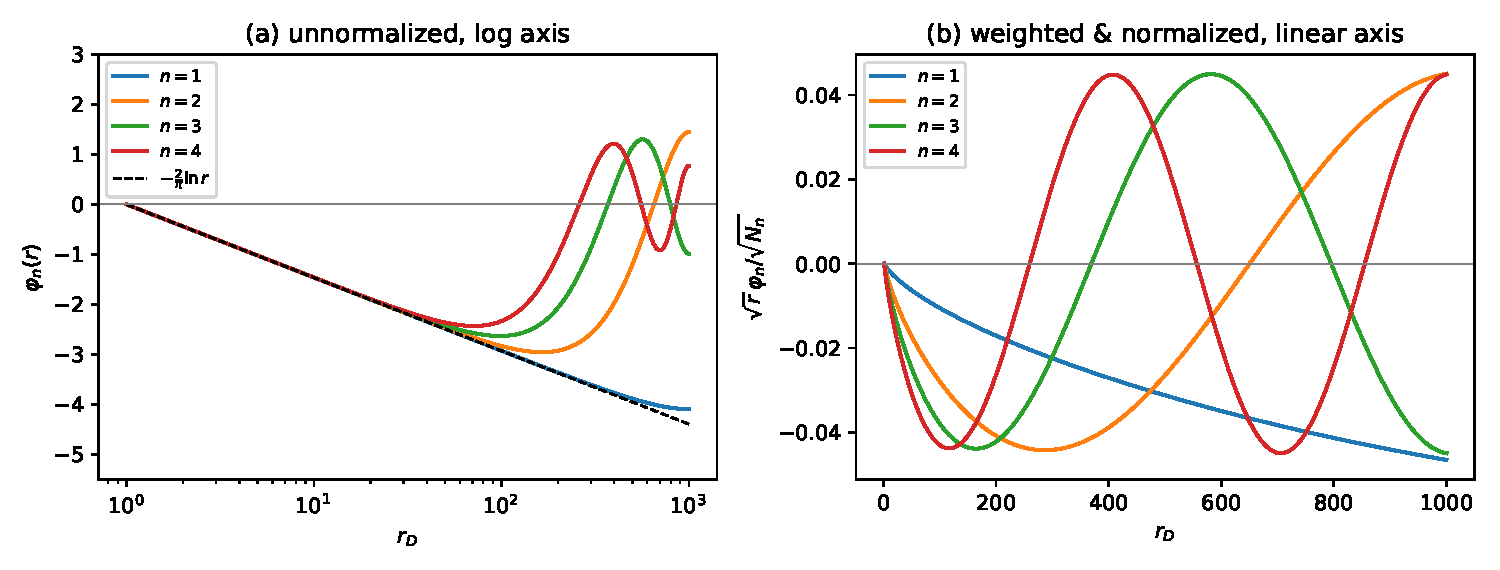
\includegraphics[width=\linewidth]{fig_phi.pdf}
  \caption{First four annular eigenfunctions for $\reD=1000$.
  (a) Unnormalized $\varphi_n$ on a log axis: all modes follow $-\frac{2}{\pi}\ln r$ near the well and
  separate further out.
  (b) $\sqrt{r}\,\varphi_n/\sqrt{N_n}$ on a linear axis: sine-like modes of nearly equal amplitude with
  $n-1$ interior zeros and zero slope at $r=\reD$.}
  \label{fig:phi}
\end{figure}

\subsection{Orthogonality and normalization}
\begin{equation}
  \int_1^{\reD} r\,\varphi_m\varphi_n\,\dd r = N_n\,\delta_{mn},\qquad
  N_n = \frac{\reD^2}{2}\,\varphi_n(\reD)^2 - \frac{2}{\pi^2\lambda_n^2},
\end{equation}
where the second term uses the Wronskian identity $J_1(x)Y_0(x)-J_0(x)Y_1(x) = 2/(\pi x)$,
which gives $Z_1(\lambda_n) = 2/(\pi\lambda_n)$.

\subsection{Transform pair}
\begin{equation}
  \hat u_n = \mathcal{H}[u]_n = \frac{1}{N_n}\int_1^{\reD} r\,u(r)\,\varphi_n(r)\,\dd r,
  \qquad
  u(r) = \mathcal{H}^{-1}[\hat u](r) = \sum_{n=1}^{\infty}\hat u_n\,\varphi_n(r).
\end{equation}
Every truncated reconstruction $\sum_{n\le K}\hat u_n\varphi_n$ satisfies both boundary conditions exactly.

\section{Reference solutions}

\subsection{Homogeneous case ($k_D\equiv1$)}
Since $\mathcal{L}\varphi_n = -\lambda_n^2\varphi_n$, the dynamics are diagonal:
\begin{equation}
  \hat u_n(t+\Delta t) = e^{-\lambda_n^2\Delta t}\,\hat u_n(t).
  \label{eq:diag}
\end{equation}
With $u(r,0)=1$ and $\int_1^{\reD} r\varphi_n\,\dd r = -2/(\pi\lambda_n^2)$:
\begin{align}
  u(r,t) &= -\sum_{n=1}^\infty \frac{2}{\pi\lambda_n^2 N_n}\,\varphi_n(r)\,e^{-\lambda_n^2 t},\\
  q_D(t) &= \sum_{n=1}^\infty \frac{4}{\pi^2\lambda_n^2 N_n}\,e^{-\lambda_n^2 t}.
\end{align}
These are the benchmarks for validating the numerical solver. The pressure itself follows from
$p(r,t) = p_{wf} + (p_i-p_{wf})\,u(r,t)$.

\paragraph{Convergence of the series.}
Mode $n$ is damped by $e^{-\lambda_n^2 t}$, so the number of modes needed grows as $t\to0$.
Table~\ref{tab:conv} lists the number of terms required for an absolute accuracy of $10^{-3}$ in $u(2,t)$,
measured against a 1908-term reference ($\lambda_n\le6$).
\begin{center}
\begin{tabular}{@{}rcc@{}}
\toprule
$t_D$ & $u(2,t_D)$ & modes for $10^{-3}$ accuracy \\
\midrule
$10^{1}$ & 0.3687 & 190 \\
$10^{2}$ & 0.2395 & 54 \\
$10^{4}$ & 0.1358 & 5 \\
$10^{6}$ & 0.0808 & 1 \\
\bottomrule
\end{tabular}
\captionof{table}{Modes needed for the homogeneous series at $r_D=2$, $\reD=1000$.}
\label{tab:conv}
\end{center}
Late times need only a few modes. At early times the pressure front near the well is sharp and needs hundreds.
This is the series view of the early-time (Gibbs) difficulty, and it supports pairing $\Delta t=100$ with $K=32$
once $t\gtrsim100$.

\paragraph{Flow regimes.}
Figure~\ref{fig:pressure} shows the analytic solution. The pressure disturbance spreads outward roughly linearly in
$\ln r$ (infinite-acting radial flow). In this period the rate follows the classical approximation
$q_D\approx 2/(\ln t_D + 0.809)$ (e.g.\ $\approx0.20$ at $t_D=10^4$). Once the disturbance reaches $\reD$
(around $t_D\sim10^5$--$10^6$), the reservoir depletes and $q_D$ declines exponentially. In that regime the first
mode alone, $q_D\approx \frac{4}{\pi^2\lambda_1^2N_1}e^{-\lambda_1^2 t}$, reproduces the full series.

\begin{figure}[h]
  \centering
  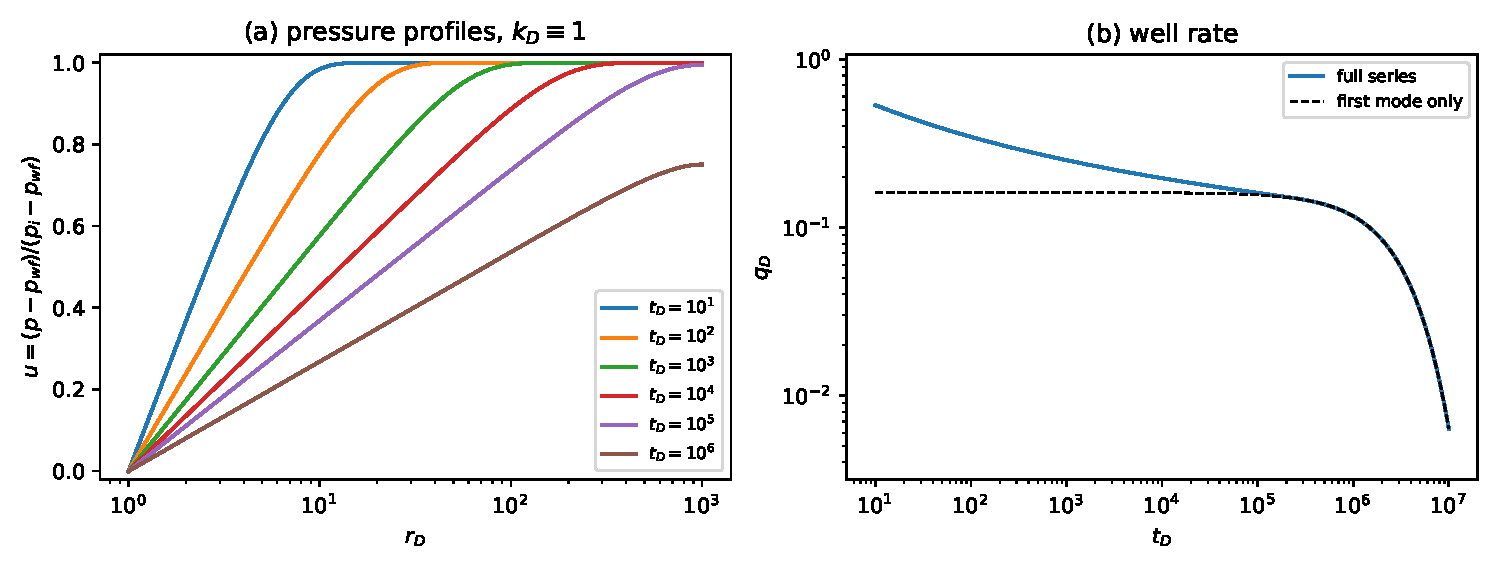
\includegraphics[width=\linewidth]{fig_pressure.pdf}
  \caption{Analytic solution for $k_D\equiv1$, $\reD=1000$ (1908 modes).
  (a) Dimensionless pressure $u=(p-p_{wf})/(p_i-p_{wf})$ at $t_D=10^1,\dots,10^6$.
  (b) Well rate $q_D(t)$: the full series compared with the first mode alone, which matches the
  boundary-dominated exponential decline.}
  \label{fig:pressure}
\end{figure}

\subsection{Heterogeneous case}
Substitute $u=\sum_n \hat u_n\varphi_n$ into \eqref{eq:pde}, project onto $\varphi_m$ with weight $r$, and integrate
by parts. The boundary terms vanish because $\varphi_m(1)=0$ and $u'(\reD)=0$. The result is
\begin{equation}
  \frac{\dd\hat{\mathbf u}}{\dd t} = \mathbf A(k_D)\,\hat{\mathbf u},\qquad
  A_{mn}(k_D) = -\frac{1}{N_m}\int_1^{\reD} r\,k_D(r)\,\varphi_m'(r)\,\varphi_n'(r)\,\dd r,
\end{equation}
so the exact one-step map is
\begin{equation}
  \hat{\mathbf u}(t+\Delta t) = \exp\!\big(\Delta t\,\mathbf A(k_D)\big)\,\hat{\mathbf u}(t).
  \label{eq:expA}
\end{equation}
For $k_D\equiv1$, $\mathbf A = -\operatorname{diag}(\lambda_n^2)$ and \eqref{eq:expA} reduces to \eqref{eq:diag}.
For heterogeneous $k_D$, $\mathbf A$ is dense, so permeability couples the modes. The operator to learn is linear in $u$
and nonlinear in $k_D$: the network must learn $k_D\mapsto \exp(\Delta t\,\mathbf A(k_D))$.
This motivates spectral layers that act on the Hankel coefficients.

\section{Learning problem}

\subsection{Operator}
\begin{equation}
  \mathcal{G}:\ \big(u(\cdot,t),\ \ln k_D(\cdot)\big)\ \longmapsto\ u(\cdot,t+\Delta t),
\end{equation}
with fixed $\Delta t = 100$. Full trajectories are obtained by autoregressive rollout
$u^{(j+1)} = \mathcal{G}_\theta(u^{(j)},\ln k_D)$.
Trajectories start at $t_0>0$, taken from the reference solver, to avoid the discontinuity between $u(r,0)=1$ and $u(1,t)=0$
(which would cause Gibbs oscillations near the well).

\paragraph{Mode truncation.} Mode $n$ is damped per step by $e^{-\lambda_n^2\Delta t}$. With $\Delta t=100$ and
$\lambda_n\approx n\pi/999$, modes $n\gtrsim 30$ are strongly damped in one step, which motivates $K=32$.

\subsection{Hankel Neural Operator architecture}
Inputs on the grid: $a(r) = \big(u(r,t),\ \ln k_D(r)\big)$, optionally with the coordinate $\ln r$.
\begin{align}
  v^{0}(r) &= P\,a(r), && P:\mathbb{R}^{d_a}\to\mathbb{R}^{C}\ \text{(lifting)},\\
  v^{\ell+1}(r) &= \sigma\!\Big( W_\ell\, v^{\ell}(r) + b_\ell + \sum_{n=1}^{K} R_{\ell,n}\,\hat v^{\ell}_n\,\varphi_n(r) \Big),
  && \ell=0,\dots,L-1,\\
  u(r,t+\Delta t) &\approx g(r)\; Q\,v^{L}(r), && Q:\mathbb{R}^{C}\to\mathbb{R}\ \text{(projection)},
\end{align}
where $\hat v^\ell_n = \mathcal{H}[v^\ell]_n$ is applied channel-wise, $R_{\ell,n}\in\mathbb{R}^{C\times C}$ are learned
\emph{real} spectral weights (the transform is real, unlike the complex weights of FNO), $W_\ell$ is a pointwise
linear map, and $\sigma$ is GELU. The factor $g(r)$ with $g(1)=0$ (e.g.\ $g=\ln r/\ln\reD$) enforces the inner
boundary condition exactly. The exact form of this hard constraint is still an open design choice.

\subsection{Discretization}
Use a log-spaced grid $x_j=\ln r_j = j\,\Delta x$, $j=0,\dots,N-1$, $\Delta x=\ln\reD/(N-1)$.
Since $r\,\dd r = r^2\,\dd x$, the quadrature weights are $w_j = c_j\, r_j^2\,\Delta x$ (trapezoidal $c_j$).
Let $\mathbf W=\operatorname{diag}(w_j)$ and define the inverse transform by sampling the eigenfunctions:
\begin{equation}
  \mathbf u = \mathbf B\,\hat{\mathbf u},\qquad B_{jn} = \varphi_n(r_j).
\end{equation}
Two choices for the forward transform $\hat{\mathbf u}=\mathbf T\mathbf u$ were compared:
\begin{align}
  \text{quadrature:}\quad & T_{nj} = \frac{w_j\,\varphi_n(r_j)}{N_n}, \\
  \text{least squares:}\quad & \mathbf T = \big(\mathbf B^{\top}\mathbf W\mathbf B\big)^{-1}\mathbf B^{\top}\mathbf W .
  \label{eq:lstsq}
\end{align}
The quadrature form discretizes the continuous transform directly, so $\mathbf T\mathbf B=\mathbf I_K$ holds only up to
the $O(\Delta x^2)$ trapezoidal error. The least-squares form is the $\mathbf W$-weighted best fit of $\mathbf u$ by
$K$ modes. It satisfies $\mathbf T\mathbf B=\mathbf I_K$ exactly, $\mathbf B\mathbf T$ is a projector, and the exact
homogeneous step \eqref{eq:diag} is reproduced to machine precision. Table~\ref{tab:grid} shows that it is also far
more accurate for functions outside the span of the $K$ modes. \textbf{The least-squares form \eqref{eq:lstsq} on a
log grid ($\alpha=1$) with $N=1024$ is adopted.}

\begin{center}
\begin{tabular}{@{}lrcc@{}}
\toprule
$\mathbf T$ & $N$ & $\max|\mathbf T\mathbf B-\mathbf I_K|$ & rel.\ error of $\mathcal H[1]$ \\
\midrule
quadrature    & 512  & $1.9\times10^{-3}$ & $1.8\times10^{-3}$ \\
quadrature    & 1024 & $4.4\times10^{-4}$ & $4.2\times10^{-4}$ \\
quadrature    & 2048 & $1.1\times10^{-4}$ & $1.0\times10^{-4}$ \\
least squares & 512  & $9\times10^{-16}$  & $9.8\times10^{-7}$ \\
least squares & 1024 & $2\times10^{-15}$  & $1.9\times10^{-7}$ \\
least squares & 2048 & $2\times10^{-15}$  & $4.5\times10^{-8}$ \\
\bottomrule
\end{tabular}
\captionof{table}{Transform accuracy on the log grid, $K=32$, $\reD=1000$ (\texttt{phase\_1/grid\_study.py}).
The error of $\mathcal H[1]$ is measured against the exact coefficients $-2/(\pi\lambda_n^2N_n)$, relative to the
largest one. A higher-order (Gregory) quadrature was also tried and was less accurate at these $N$, because products
$\varphi_m\varphi_n$ are under-resolved near $\reD$.}
\label{tab:grid}
\end{center}

$\mathbf T\in\mathbb{R}^{K\times N}$ and $\mathbf B\in\mathbb{R}^{N\times K}$ are precomputed once and stored as fixed
buffers. A spectral convolution costs $O(NKC + KC^2)$. The reconstruction error of a smooth function satisfying both
boundary conditions levels off at $\approx7\times10^{-4}$ for all grids; this is the $K=32$ truncation error, not a
discretization error.

\begin{remark}[Resolution near the outer boundary]
The log grid concentrates points near the well, but mode $K$ oscillates with wavelength $2\pi/\lambda_K$ everywhere, and
grid spacing grows like $r\,\Delta x$. Requiring $P$ points per wavelength at $r=\reD$ gives
\begin{equation}
  N \gtrsim \frac{P\,\lambda_K\,\reD\ln\reD}{2\pi}.
\end{equation}
For $K=32$ ($\lambda_K\approx0.1$), $\reD=1000$, $P=8$: $N\gtrsim 900$. With the least-squares transform this
estimate is conservative: $N=512$ already gives coefficient errors of $\sim10^{-6}$ (Table~\ref{tab:grid}).
It may still apply to the finite-volume solver, which must resolve the solution rather than the modes.
\end{remark}

\section{Data}
\label{sec:data}
Generated by \texttt{phase\_1/dataset.py}; stored in \texttt{phase\_1/data/} as \texttt{train.npz}, \texttt{val.npz} and \texttt{test.npz}.
\begin{itemize}
  \item \textbf{Permeability:} $\ln k_D(r) = m + \xi(\ln r) + s\,\mathbb 1[r<r_s]$, clipped to $[-3,3]$.
        The mean shift is $m\sim\mathcal N(0,0.3^2)$. The field $\xi$ is a zero-mean Gaussian random field in $x=\ln r$
        with squared-exponential covariance $\sigma^2 e^{-(x-x')^2/(2\ell^2)}$, $\sigma\sim U(0.5,1)$, $\ell\sim U(0.3,1.5)$.
        With probability $0.5$ a near-well skin offset $s=\ln(k_s/k)\sim U(\ln0.1,\ln5)$ applies for
        $r<r_s$, $r_s$ log-uniform in $[2,20]$. About $3.5\%$ of the fields reach the clip.
  \item \textbf{Reference solver:} vertex-centered finite volumes on the $N=1024$ log grid, face fluxes exact for
        $u$ linear in $\ln r$, harmonic-mean face permeability, variable-step BDF2 (largest step 20).
        For $k_D\equiv1$ the error against the series of Section~3.1 is $\sim4\times10^{-7}$ for $t_D\ge10^4$.
  \item \textbf{Trajectories:} from $u=1$ at $t_D=0$ (so the surrogate never needs the solver), stored every
        $\Delta t_D=1000$ up to $5\times10^5$ (501 states). With $\Delta t_D=1000$ and $K=32$ the exact first step from
        $u=1$ is representable to $3\times10^{-7}$ ($1.5\times10^{-2}$ at $\Delta t_D=100$).
        Training pairs $\big((u^{(j)},\ln k_D),\,u^{(j+1)}\big)$ are formed from consecutive states.
  \item \textbf{Size:} 800 / 100 / 100 trajectories (train / validation / test, seeds 0 / 1 / 2), float32, about 2\,GB.
\end{itemize}

\paragraph{Near-well structure.}
The flux $r k_D\,\partial_r u$ varies smoothly in $r$, so $\partial_r u \propto 1/k_D$ and every near-well permeability
feature leaves a kink in $u$ that diffusion does not remove. The $K=32$ eigenfunctions of the $k_D\equiv1$ problem have a
shortest wavelength of about $2\pi/\lambda_{32}\approx 64$ in $r$ and cannot represent it
(Figure~\ref{fig:dataset}d--f). At $t_D=5\times10^4$ the relative $L_2$ error of the 32-mode projection has median
$4.5\%$ ($3.9\%$ without skin, $5.4\%$ with skin) and 90th percentile $11\%$; $94\%$ of the residual lies at $r<10$.
For $k_D\equiv1$ the same error is below $10^{-6}$ from $t_D=10^3$. The near-well detail must therefore be carried by
the pointwise path of the network, and an FNO-1D on the log grid (modes spread evenly in $\ln r$) may be a strong
baseline.

\begin{figure}[h]
  \centering
  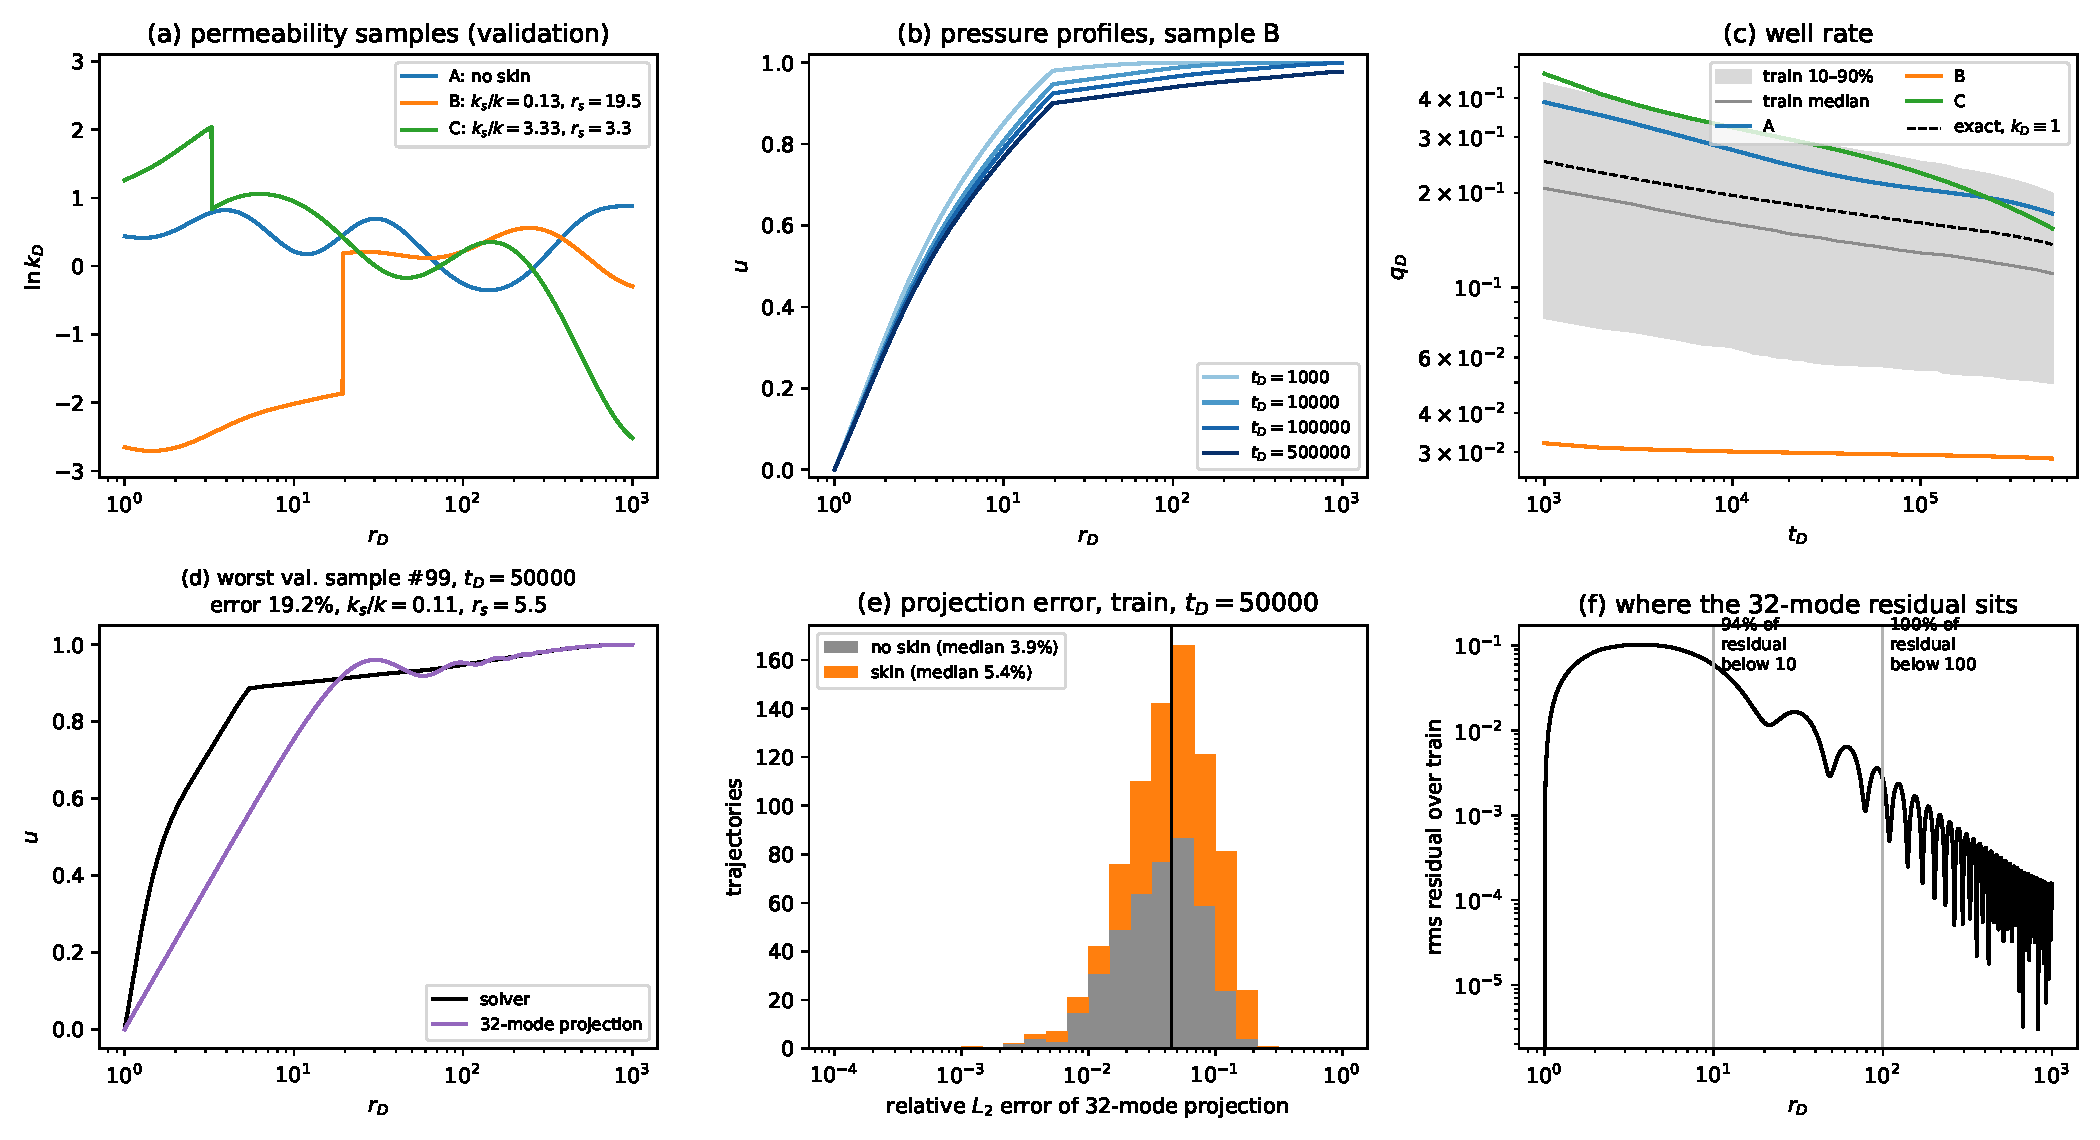
\includegraphics[width=\linewidth]{fig_dataset.pdf}
  \caption{Dataset overview.
  (a) Three validation permeability fields: no skin, damaged well, stimulated well.
  (b) Pressure profiles of the damaged-well sample.
  (c) Well rate of the three samples, 10--90\% band and median over the training set, and the exact $k_D\equiv1$ rate.
  (d) Worst validation state at $t_D=5\times10^4$ and its 32-mode projection.
  (e) Projection error over the training set.
  (f) Root-mean-square projection residual versus $r$.}
  \label{fig:dataset}
\end{figure}

\section{Evaluation}
\begin{itemize}
  \item One-step relative error in the weighted norm
        $\|e\|^2_r = \int_1^{\reD} r\,e^2\,\dd r$, i.e.\ $\|u_\theta-u\|_r/\|u\|_r$.
  \item Rollout error over a limited horizon (about 100--500 steps).
  \item Well-rate error in $q_D(t)$.
  \item Baseline: FNO-1D trained on the same data.
  \item Transform tests: $\mathbf T\mathbf B\approx \mathbf I_K$; orthogonality; for $k_D\equiv1$, one HNO spectral layer
        with $R_n=e^{-\lambda_n^2\Delta t}$ reproduces \eqref{eq:diag} exactly.
\end{itemize}

\section{Summary of phase-1 choices}
\begin{center}
\begin{tabular}{@{}ll@{}}
\toprule
Item & Choice \\
\midrule
Geometry & $\reD=1000$ (fixed) \\
Varying input & $k_D(r)$ only \\
Operator & $(u_t,\ln k_D)\mapsto u_{t+\Delta t}$ \\
Time step & $\Delta t_D = 1000$, 500 steps to $t_D=5\times10^5$ (later an input channel) \\
Initial state & $u=1$ at $t_D=0$ \\
Data & 800 / 100 / 100 trajectories, Section~\ref{sec:data} \\
Spectral modes & $K=32$ \\
Basis & annular $J_0/Y_0$ eigenfunctions, eq.~\eqref{eq:eig} \\
Grid & log-spaced in $r_D$, $N=1024$ \\
Transform & least squares, eq.~\eqref{eq:lstsq} \\
Stack & PyTorch + SciPy \\
\bottomrule
\end{tabular}
\end{center}

\end{document}
